\chapter{数学基础}\label{chap:math-basics}
\addtocontents{los}{\protect\addvspace{10pt}}

\begin{intro}
物理的学习离不开数学,但学习时间的有限使得很多同学纠结数学应该学到多深。在普通物理的范畴内,作者在这里提出一些小小的建议。

数学知识分两类。

第一类是需要完全理解和掌握的,比如数列、导数和积分、微分方程……它们在题目中出现的概率很高,当我们遇到时要能从容应对。

第二类是有助于物理理解,但不要求完全掌握的,比如矢量分析与场论、张量代数……它们有助于加深你对物理情景的理解,但在普通物理的题目中出现的概率较低,这种知识需要学习,但学习的深度要视自身情况而定。

这一章虽然叫做数学基础,篇幅不长,但涵盖的内容并不少,并不需要通篇阅读,而是当你在学习物理的过程中遇到了数学上的困难时,再回头查阅有关内容。
如果你能从我的注记中获得一些启发,那我的目的便达到了。
\end{intro}

\section{一元函数微积分}\label{sec:single-variable-calculus}

\subsection{微分}\label{subsec:differential}

一元函数可记为
\begin{equation*}
    y = y(x)\ \text{或}\ y = f(x),
\end{equation*}

在它的连续区间内,如图 \ref{fig:function-increment}

\input{figure/chap.00/fig.function-increment.tex}

所示,自变量由 $x$ 变到 $x + \Delta x$,相应的,$y$ 由 $y(x)$ 变到 $y(x + \Delta x)$,则函数的增量定义为
\begin{equation*}
    \Delta y = y(x + \Delta x) - y(x).
\end{equation*}

自变量 $ \Delta x \to 0$ 时,称为自变量微分,记为 $ \d x$,$ \d x$ 是无穷小量,不是零。
但因为它是无穷小量,它在与有限量的运算中,在一些情况下可以视为 0 (但不是在所有情况下都可以视为 0)。
在连续区间内,自变量增量 $\Delta x$ 趋近于微分 $\d x$,函数增量 $\Delta y \to \d y$,称为函数微分,记为 $\d y$,它也是无穷小量。
$ \d y $ 与 $ \d x $ 之间的关系为
\begin{equation*}
    \d y = y (x + \d x) - y (x).
\end{equation*}

\begin{note}{符号说明}{symbol-explanation}
    显然,因为 $ y(x) $ 不一定是单调函数,所以 $ \Delta y $ 和 $ \d y $ 可以是正的、负的或零。
    所以只要你严格遵守定义与符号计算的基本规则,就不会出错。
    这句话在一些微元分析的场景下尤其适用。
\end{note}

\begin{example}{重要近似}{important-approximation}
    \begin{equation}
        \sin x \sim \tan x \sim x, (x \to 0).
    \end{equation}
    证明:

    \input{figure/chap.00/fig.important-approximation.tex}

    以 $ O $ 为原点建立直角坐标系,绘出以 $ R $ 为半径的圆弧如图 \ref{fig:important-approximation} 所示,
    其中圆心角 $ \theta $ 对应的直线段 $ AA' $ ,$ BB' $ ,圆弧 $ \wideparen{AB} $ 的长度分别为
    \begin{equation*}
        \overline{AA'} = R \sin \theta, \quad \overline{BB'} = R \tan \theta, \quad \wideparen{AB} = R \theta.
    \end{equation*}

    $\theta \to 0$ 时,有
    \begin{equation*}
        \overline{AA'} \sim \overline{BB'} \sim \wideparen{AB} .
    \end{equation*}

    化简得
    \begin{equation*}
        \sin \theta \sim \tan \theta \sim \theta, (\theta \to 0).
    \end{equation*}
    \qed
\end{example}

\subsection{导数}\label{subsec:derivative}

\begin{definition}{导数}{derivative}
    函数 $ y = f(x) $ 在点 $ x $ 处的导数定义为
    \begin{equation}
        f'(x) = \lim_{\Delta x \to 0} \frac{\Delta y}{\Delta x} = \lim_{\Delta x \to 0} \frac{f(x + \Delta x) - f(x)}{\Delta x},
    \end{equation}

    如果极限存在,则称函数在点 $ x $ 处可导。
    
\end{definition}

显然,导数的几何意义是函数图像在点 $ (x, f(x)) $ 处的切线的斜率。
\bigskip

在数学上可以证明导数与微分有如下关系:
\begin{definition}{微分与导数的关系}{differential-derivative-relation}
    函数 $ y = f(x) $ 在点 $ x $ 处可导,则函数在该点的微分与导数的关系为
    \begin{equation}
        \d y = f'(x) \d x.
    \end{equation}

    因此,导数也称为函数的微商,而求导和求微分实际上是等价的。

\end{definition}

\begin{note}{导数与微分的区别}{derivative-differential-difference}
    导数是一个极限值,是一个确定的数值,而微分是函数增量的线性主部,不是一个确定的数值。
    导数表示函数在某点处的变化率,而微分表示函数在该点处变化量的线性近似。
    \medskip

    并且导数不能视为 $ \d y $ 与 $ \d x $的比值,这只是 Leibniz 记号下的一个形式上的表示方法。
    当然,在非严格的物理推导中,我们经常会把导数视为 $ \d y $ 与 $ \d x $ 的比值来进行计算。
    并且可以用类似的方法处理常微分中的微元计算,这种做法(形式计算)在物理学中是被广泛接受的。
    \medskip

    当然,如果从更高级的数学角度来看,我们的操作是有严格依据的,这也保证了我们不会出错,这里便不再深入了。

\end{note}

导数有一些重要性质,举例如下:
\begin{illustration}{导数的性质}{derivative-properties}
    \begin{align}
        &(1)\quad (A_1 y_1 + A_2 y_2)' = A_1 y_1' + A_2 y_2' ;\\
        &(2)\quad (y_1 y_2)' = y_1' y_2 + y_1 y_2' ;\\
        &(3)\quad \left( \frac{y_1}{y_2} \right)' = \frac{y_1' y_2 - y_1 y_2'}{y_2^2} ;\\
        &(4)\quad (y_1 \circ y_2)' = (y_1' \circ y_2) \cdot y_2' .\label{eq:derivative-composition}
    \end{align}

\end{illustration}

证明略去。

其中,式 \ref{eq:derivative-composition} 被称为复合函数的求导法则。
在微分的形式下,式 \ref{eq:derivative-composition} 可写为
\begin{equation}
    \frac{\d y_2}{\d x} = \frac{\d y_2}{\d y_1} \cdot \frac{\d y_1}{\d x}.
\end{equation}

这也在一定程度上为我们对导数执行的“消去”操作的正确性提供了依据。
\bigskip

常用的导数公式列举如下:
\begin{illustration}{常用导数公式}{common-derivative-formulas}
    \begin{align}
        &(1)\quad (x^n)' = n x^{n-1} ;\\
        &(2)\quad (a^x)' = a^x \ln a ;\\
        &(3)\quad (\log _a x)' = \frac{1}{x \ln a} ;\\
        &(4)\quad (\sin x)' = \cos x ;\\
        &(5)\quad (\cos x)' = -\sin x ;\\
    \end{align}

\end{illustration}

此外,还有几个常用的 $ n $ 阶导数公式:
\begin{illustration}{常用 $ n $ 阶导数公式}{common-nth-derivative-formulas}
    \begin{align}
        &(1)\quad (e^{a x})^{(n)} = a^n e^{a x} ;\\
        &(2)\quad (\sin a x)^{(n)} = a^n \sin \left( a x + \frac{n \pi}{2} \right) ;\\
        &(3)\quad (\cos a x)^{(n)} = a^n \cos \left( a x + \frac{n \pi}{2} \right) .
    \end{align}

\end{illustration}

在数学上,导数还可以用来讨论函数曲线的极值位置与凹凸性,这在物理中经常用到,而且有如下结论:
\begin{definition}{极值与凹凸性的判定}{extreme-concavity-determination}
    设函数 $ y = f(x) $ 在点 $ x_0 $ 处可导,且 $ f'(x_0) = 0 $。
    \begin{itemize}
        \item 若 $ f''(x_0) > 0 $,则 $ f(x) $ 在点 $ x_0 $ 处取得极小值,且曲线在该点处向下凸,称为“凸”;
        \item 若 $ f''(x_0) < 0 $,则 $ f(x) $ 在点 $ x_0 $ 处取得极大值,且曲线在该点处向上凸,称为“凹”;
        \item 若 $ f''(x_0) = 0 $,则不能确定 $ f(x) $ 在点 $ x_0 $ 处是否取得极值,需考察更高阶导数。
    \end{itemize}

    注意到,函数的凹凸与“凹”“凸”这两个字的字型是相反的,这是因为函数的凸性与凸集有关,而凸集的定义是明确的,因此相反。

\end{definition}

接下来,我们介绍与导数有关的另一个重要工具——泰勒公式。
\begin{theorem}{泰勒公式}{taylor-formula}
    设函数 $ y = f(x) $ 在点 $ x_0 $ 处具有 $ n + 1 $ 阶导数,则在点 $ x_0 $ 附近,函数 $ f(x) $ 可展开为
    \begin{equation}
        f(x) = f(x_0) + \frac{f'(x_0)}{1!} (x - x_0) + \frac{f''(x_0)}{2!} (x - x_0)^2 + \cdots + \frac{f^{(n)}(x_0)}{n!} (x - x_0)^n + R_n,
    \end{equation}

    其中,余项 $ R_n $ 有如下两种形式:
    \begin{itemize}
        \item 拉格朗日(Lagrange)余项形式:
        \begin{equation}
            R_n = \frac{f^{(n+1)}(\xi)}{(n+1)!} (x - x_0)^{n+1},\quad \xi\text{ 在 } x \text{ 与 } x_0 \text{ 之间} ;
        \end{equation}
        \item 皮亚诺(Peano)余项形式:
        \begin{equation}
            R_n = o \left( (x - x_0)^n \right),\quad x \to x_0 .
        \end{equation}
    \end{itemize}
    
\end{theorem}

泰勒公式表明,函数在某点处的值可以用该点处的各阶导数来近似表示。
上述定义中的余项 $ R_n $ 描述了近似的误差大小。
对于物理问题,我们通常只需要前几项的近似,因此余项的具体形式并不重要,我们也不必过多纠结。

显然,函数如果想展成泰勒级数,至少要求通项趋于零,即
\begin{equation*}
    \lim_{n \to \infty} \frac{f^{(n)}(x_0)}{n!} (x - x_0)^n = 0.
\end{equation*}

但事实上,函数能否展成泰勒级数,还需要满足更强的条件,这里不再赘述。
\bigskip

函数 $ f(x) $ 若能在点 $ x_0 $ 两侧某范围内展开成泰勒级数,且级数在该范围内收敛于函数值,便称这一范围为 $ f(x) $ 的收敛区间。
例如,在数学上可以证明:
\begin{illustration}{常见函数的泰勒展开}{common-function-taylor-expansion}
    \begin{align}
        &(1)\quad e^x = \sum_{n=0}^{\infty} \frac{x^n}{n!},\quad x \in (-\infty, +\infty) ;\\
        &(2)\quad \sin x = \sum_{n=0}^{\infty} (-1)^n \frac{x^{2n+1}}{(2n+1)!},\quad x \in (-\infty, +\infty) ;\\
        &(3)\quad \cos x = \sum_{n=0}^{\infty} (-1)^n \frac{x^{2n}}{(2n)!},\quad x \in (-\infty, +\infty) ;\\
        &(4)\quad \ln (1 + x) = \sum_{n=1}^{\infty} (-1)^{n-1} \frac{x^n}{n},\quad x \in (-1, 1] ;\\
        &(5)\quad (1 + x)^m = \sum_{n=0}^{\infty} \binom{m}{n} x^n,\quad x \in (-1, 1) .\label{eq:taylor-binomial}
    \end{align}
    
\end{illustration}

其中,式 \ref{eq:taylor-binomial} 中的二项式系数定义为
\begin{equation}
    \binom{m}{n} = \frac{m (m - 1) (m - 2) \cdots [m - (n - 1)]}{n!}.
\end{equation}

$ x_0 = 0 $ 时,称为麦克劳林(Maclaurin)级数。

\subsection{积分}\label{subsec:integral}

有许多数学书上把积分分为了不定积分与定积分两类,还有“积分是导数的逆运算”这样的说法。

但实际上,积分的本质是求和,而我更愿意把求不定积分看作是求原函数的问题,而把定积分视为真正意义上的“积分”,即求和。

\begin{definition}{不定积分}{indefinite-integral}
    设函数 $ F(x) $ 的导数为 $ f(x) $,即 $ F'(x) = f(x) $,则称函数 $ F(x) $ 为函数 $ f(x) $ 的一个原函数。
    函数 $ f(x) $ 的所有原函数的集合称为函数 $ f(x) $ 的不定积分,记为
    \begin{equation*}
        \int f(x) \d x = F(x) + C,
    \end{equation*}

    其中,$ C $ 为任意常数。
\end{definition}

根据 \cref{illustration:derivative-properties} 中导数的性质,可以得到不定积分的一些性质,举例如下:
\begin{illustration}{不定积分的性质}{indefinite-integral-properties}
    \begin{align}
        &(1)\quad \int [A_1 f_1(x) + A_2 f_2(x)] \d x = A_1 \int f_1(x) \d x + A_2 \int f_2(x) \d x ;\\
        &(2)\quad \int f'(x) g(x) \d x = f(x) g(x) - \int f(x) g'(x) \d x ;\\
        &(3)\quad \int f(g(x)) g'(x) \d x = \int f(u) \d u,\quad u = g(x) .
    \end{align}

\end{illustration}

同时,根据 \cref{illustration:common-derivative-formulas} 中常用的导数公式,可以得到一些常见函数的不定积分,举例如下:
\begin{illustration}{常见函数的不定积分}{common-indefinite-integral}
    \begin{align}
        &(1)\quad \int x^n \d x = \frac{x^{n+1}}{n+1} + C,\quad (n \neq -1) ;\\
        &(2)\quad \int \frac{1}{x} \d x = \ln |x| + C ;\\
        &(3)\quad \int a^x \d x = \frac{a^x}{\ln a} + C ;\\
        &(4)\quad \int \log_a x \d x = x (\log_a x - \log_e a) + C ;\\
        &(5)\quad \int \sin x \d x = -\cos x + C ;\\
        &(6)\quad \int \cos x \d x = \sin x + C .
    \end{align}

\end{illustration}

有了这些,我们就可以计算几乎所有可解的不定积分了。
\bigskip

\begin{definition}{定积分}{definite-integral}
    设函数 $ f(x) $ 在区间 $ [a, b] $ 上有定义,且在该区间上可积,则称
    \begin{equation}
        \int_a^b f(x) \d x = \lim_{n \to \infty} \sum_{i=1}^n f(\xi_i) \Delta x_i,
    \end{equation}

    其中,区间 $ [a, b] $ 被分成 $ n $ 个子区间 $ [x_{i-1}, x_i] $,$ \Delta x_i = x_i - x_{i-1} $,$ \xi_i \in [x_{i-1}, x_i] $。
    若极限存在,则称该极限为函数 $ f(x) $ 在区间 $ [a, b] $ 上的定积分。
    
\end{definition}

这是定积分的黎曼(Riemann)定义,它的几何意义是曲线 $ y = f(x) $ 与 $ x $ 轴及直线 $ x = a $ 和 $ x = b $ 所围成的面积(注意符号)。
但是这个定义在实际计算中并不实用,我们需要借助不定积分来计算定积分(这也正是不定积分这个概念被提出的原因)。

这就需要用到著名的微积分基本定理。

\begin{theorem}{微积分基本定理}{fundamental-theorem-of-calculus}
    设函数 $ f(x) $ 在区间 $ [a, b] $ 上连续,且 $ F(x) $ 是 $ f(x) $ 的一个原函数,则
    \begin{equation}
        \int_a^b f(x) \d x = F(b) - F(a).
    \end{equation}

    证明:

    设区间 $ [a, b] $ 被分成 $ n $ 个子区间 $ [x_{i-1}, x_i] $,$ \Delta x_i = x_i - x_{i-1} $,$ \xi_i \in [x_{i-1}, x_i] $。
    则有
    \begin{equation*}
        \sum_{i=1}^n f(\xi_i) \Delta x_i = \sum_{i=1}^n [F(x_i) - F(x_{i-1})] = F(b) - F(a).
    \end{equation*}
    当 $ n \to \infty $ 时,右端不变,因此
    \begin{equation*}
        \int_a^b f(x) \d x = F(b) - F(a).
    \end{equation*}
    \qed
    上述证明中运用了微分中值定理,亦即拉格朗日(Lagrange)中值定理,可以自行查阅相关资料,此处不再赘述。
\end{theorem}

由此,我们可以通过求不定积分来计算定积分了。

类似于不定积分,定积分也有一些性质,举例如下:
\begin{illustration}{定积分的性质}{definite-integral-properties}
    \begin{align}
        &(1)\quad \int_a^b [A_1 f_1(x) + A_2 f_2(x)] \d x = A_1 \int_a^b f_1(x) \d x + A_2 \int_a^b f_2(x) \d x ;\\
        &(2)\quad \int_a^b f(x) \d x = -\int_b^a f(x) \d x ;\\
        &(3)\quad \int_a^b f(x) \d x = \int_a^c f(x) \d x + \int_c^b f(x) \d x .
    \end{align}
\end{illustration}

\begin{note}{积分变量的选择}{integration-variable-choice}
    在积分运算中,积分变量是一个“虚拟变量”,它可以是任何符号,只要在积分式中前后一致即可。
    例如,下面两个积分式是等价的:
    \begin{equation*}
        \int_a^b f(x) \d x = \int_a^b f(t) \d t .
    \end{equation*}
    这是因为积分变量只是一个占位符号,并不影响积分的结果。
\end{note}

下面给出一个定积分计算的例子,即曲线段长度的计算。
\begin{example}{曲线段长度}{curve-length}
    设函数 $ y = f(x) $ 在区间 $ [a, b] $ 上连续且可导,求曲线 $ y = f(x) $ 在区间 $ [a, b] $ 上的弧长。

    证明:

    设区间 $ [a, b] $ 被分成 $ n $ 个子区间 $ [x_{i-1}, x_i] $,$ \Delta x_i = x_i - x_{i-1} $,$ \xi_i \in [x_{i-1}, x_i] $。
    则曲线段在子区间 $ [x_{i-1}, x_i] $ 上的弧长近似为
    \begin{equation*}
        \Delta s_i = \sqrt{(\Delta x_i)^2 + (\Delta y_i)^2} = \sqrt{1 + \left( \frac{\Delta y_i}{\Delta x_i} \right)^2} \Delta x_i.
    \end{equation*}

    当子区间足够小时,有
    \begin{equation*}
        \frac{\Delta y_i}{\Delta x_i} \approx f'(\xi_i).
    \end{equation*}

    因此,曲线段在区间 $ [a, b] $ 上的弧长近似为
    \begin{equation*}
        S \approx \sum_{i=1}^n \sqrt{1 + [f'(\xi_i)]^2} \Delta x_i.
    \end{equation*}

    当子区间无限细分时,近似变为等于,即
    \begin{equation*}
        S = \int_a^b \sqrt{1 + [f'(x)]^2} \d x.
    \end{equation*}
    \qed
\end{example}

\begin{note}{微分形式下的曲线段长度}{differential-form-curve-length}
    在一些书上也有类似于下面的表达式:
    \begin{equation*}
        \d s = \sqrt {(\d x)^2 + (\d y)^2} = \sqrt {1 + \left( \frac{\d y}{\d x} \right)^2} \d x
    \end{equation*}

    这种表达式其实是对微分形式的曲线段长度公式的非严格表达,但也是形式计算奏效的一个例子。
\end{note}
    
\subsection{常微分方程}\label{subsec:ordinary-differential-equation}

\begin{definition}{常微分方程}{ordinary-differential-equation}
    设未知函数 $ y = y(x) $ 及其各阶导数 $ y', y'', \ldots , y^{(n)} $ 之间存在某种关系,可表示为
    \begin{equation}
        F(x, y, y', y'', \ldots , y^{(n)}) = 0,
    \end{equation}

    则称该方程为 $ n $ 阶常微分方程。
    方程中所含未知函数微商的最高阶数 $ n $ 称为微分方程的阶数。
    若方程关于 $ y , y', y'', \ldots , y^{(n)} $ 均是一次的,则称该微分方程为( $ n $ 阶)线性微分方程。
\end{definition}

一个函数 $ y = y(x) $ 若在某区间内具有 $ n $ 阶导数,且把该函数及其各阶导数代入微分方程后能使方程成立,则称该函数为该微分方程在该区间内的一个解。
因此当给定方程后,最基本的事情当然是求出方程的解,即求未知函数 $ y = y(x) $。

从数学上看,微分方程解的个数一般不唯一。
例如,最简单的一阶微分方程
\begin{equation}
    \frac{\d y}{\d x} = f(x)
\end{equation}
的通解为
\begin{equation}
    y = \int f(x) \d x = F(x) + C,
\end{equation}
其中, $ F(x) $ 是 $ f(x) $ 的一个原函数,$ C $ 为任意常数。
即对任意的常数 $ C $,函数 $ y = F(x) + C $ 都是该微分方程的一个解。
故称这样形式的解为该微分方程的“通解”。

如果事先要求解必须满足某些条件(初始条件或边界条件),比如未知函数在一个特定的 $ x_0 $ 处的值 $ y(x_0) = y_0 $,则符合要求的解
\begin{equation}
    y = \int_{x_0}^{x} f(x) \d x + y_0
\end{equation}
是唯一的,称为该微分方程的“特解”。

对于一般形式的 $ n $ 阶微分方程
\begin{equation}
    F(x, y, y', y'', \ldots , y^{(n)}) = 0,
\end{equation}
它的通解通常包含 $ n $ 个独立的任意常数 $ C_1, C_2, \ldots , C_n $。
它的解无论是隐表示 $ \Phi (x, y, C_1, C_2, \ldots , C_n) = 0 $ 还是显表示 $ y = y(x, C_1, C_2, \ldots , C_n) $,都称为该微分方程的通解或通积分。
常数 $ C_1, C_2, \ldots , C_n $ 称为积分常数。
而下列初值条件
\begin{equation}
    y(x_0) = y_0, \quad y'(x_0) = y_1, \quad \ldots , \quad y^{(n-1)}(x_0) = y_{n-1}
\end{equation}
一般来说决定了方程的一个特解。

从上面的讨论可以看出,求解微分方程的过程实际上就是一个积分的过程。
所以若微分方程的通解能用初等函数及初等函数的不定积分表示,则称方程为可积微分方程,而导出这种解的方法称为初等积分法。

然而,能用初等积分法求解的微分方程只是微分方程中的一小部分,大部分方程的求解都比较复杂,甚至没有解析解。
尽管如此这一基本方法在微分方程乃至物理学中仍然是非常重要的。
我们将会简要介绍一些用初等积分法求解微分方程的解法。
而对于(常)微分方程的一般理论,这里便不再深入了。
\bigskip

首先,我们介绍可分离变量的微分方程。
\begin{definition}{可分离变量的微分方程}{separable-variable-ordinary-differential-equation}
    设微分方程可化为如下形式:
    \begin{equation}
        \frac{\d y}{\d x} = g(x) h(y),
    \end{equation}

    则称该微分方程为可分离变量的微分方程。
\end{definition}

求解该类微分方程的方法如下:
\begin{enumerate}
    \item 若 $ h(y) = 0 $ 有解 $ y = y_0 $,则 $ y = y_0 $ 是该微分方程的一个解;
    \item 当 $ h(y) \neq 0 $ 时,可将方程变形为
    \begin{equation}
        \frac{1}{h(y)} \d y = g(x) \d x,
    \end{equation}
    然后对两边分别积分,得
    \begin{equation}
        \int \frac{1}{h(y)} \d y = \int g(x) \d x + C,
    \end{equation}
    其中,$ C $ 为任意常数。
    由此可得该微分方程的通解。
\end{enumerate}
\bigskip

其次,我们介绍齐次微分方程。
首先,我们给出齐次函数的定义。
\begin{definition}{齐次函数}{homogeneous-function}
    设函数 $ f(x, y) $ 满足如下条件:
    \begin{equation}
        f(tx, ty) = t^n f(x, y),
    \end{equation}

    其中,$ t $ 为任意常数,$ n $ 为非负整数,则称函数 $ f(x, y) $ 为 $ n $ 阶齐次函数。
\end{definition}

基于齐次函数的定义,我们可以给出齐次微分方程的定义。

\begin{definition}{齐次微分方程}{homogeneous-ordinary-differential-equation}
    对于一阶微分方程
    \begin{equation}
        P (x, y) \d x + Q (x, y) \d y = 0,
    \end{equation}
    称为齐次的,当且仅当 $ P (x, y) $ 与 $ Q (x, y) $ 均为同阶齐次函数。
    现在 $ \frac{ P (x, y) }{ Q (x, y) } $ 为零阶齐次函数,因此可化为 $ \varphi \left( \frac{y}{x} \right) $ 的形式。
    于是该微分方程可化为如下形式:
    \begin{equation}
        \frac{\d y}{\d x} = \varphi \left( \frac{y}{x} \right),
    \end{equation}
    而称该微分方程为齐次微分方程。
\end{definition}

求解该类微分方程的方法如下:
\begin{enumerate}
    \item 作变量代换 $ u = \frac{y}{x} $,则 $ y = u x $,从而有
    \begin{equation*}
        \frac{\d y}{\d x} = u + x \frac{\d u}{\d x} .
    \end{equation*}
    \item 将上式代入微分方程,得
    \begin{equation*}
        u + x \frac{\d u}{\d x} = \varphi (u) ,
    \end{equation*}
    即
    \begin{equation*}
        x \frac{\d u}{\d x} = \varphi (u) - u .
    \end{equation*}
    \item 分离变量,得
    \begin{equation*}
        \frac{1}{\varphi (u) - u} \d u = \frac{1}{x} \d x .
    \end{equation*}
    然后对两边分别积分,得
    \begin{equation*}
        \int \frac{1}{\varphi (u) - u} \d u = \int \frac{1}{x} \d x + C ,
    \end{equation*}
    其中,$ C $ 为任意常数。
    由此可得该微分方程的通解。
\end{enumerate}
\bigskip

最后,我们介绍一阶线性微分方程

\begin{definition}{一阶线性微分方程}{first-order-linear-ordinary-differential-equation}
    对于一阶微分方程,若未知函数 $ y $ 及其导数 $ \frac{\d y}{\d x} $ 都是一次的,则称该微分方程为一阶线性微分方程。
    它可化为标准形式:
    \begin{equation}
        \frac{\d y}{\d x} + P(x) y = Q(x) \label{eq:first-order-linear-ordinary-differential-equation},
    \end{equation}
    其中,$ P(x) $ 与 $ Q(x) $ 为已知函数。若右端的 $ Q(x) = 0 $,则称该微分方程为(一阶)线性齐次微分方程,否则称为(一阶)线性非齐次微分方程。
    注意到,这里的“齐次”与前面介绍的齐次微分方程的“齐次”是不同的概念。
\end{definition}

求解该类微分方程的方法如下:
\begin{enumerate}
    \item 求解对应的齐次方程
    \begin{equation*}
        \frac{\d y}{\d x} + P(x) y = 0 ,
    \end{equation*}
    它的通解为
    \begin{equation}
        y_h = C e^{-\int P(x) \d x} \label{eq:first-order-linear-ordinary-differential-equation-general-solution},
    \end{equation}
    其中,$ C $ 为任意常数。
    \item 求该非齐次方程的一个特解 $ y_p $,可用如下方法求解,即设
    \begin{equation}
        y_p = u(x) e^{-\int P(x) \d x} \label{eq:particular-solution-ansatz},
    \end{equation}
    其中,$ u(x) $ 为待定函数。
    将 $ y_p $ 代入非齐次方程,得
    \begin{equation*}
        \frac{\d u}{\d x} = Q(x) e^{\int P(x) \d x} .
    \end{equation*}
    分离变量并积分,得
    \begin{equation*}
        u(x) = \int Q(x) e^{\int P(x) \d x} \d x .
    \end{equation*}
    因此,非齐次方程的一个特解为
    \begin{equation}
        y_p = e^{-\int P(x) \d x} \int Q(x) e^{\int P(x) \d x} \d x .
    \end{equation}
    \item 由此可得该非齐次微分方程的通解为
    \begin{equation}
        y = y_h + y_p = C e^{-\int P(x) \d x} + e^{-\int P(x) \d x} \int Q(x) e^{\int P(x) \d x} \d x \label{eq:first-order-linear-ordinary-differential-equation-general-solution-nonhomogeneous}.
    \end{equation} 
\end{enumerate}

比较,式 \ref{eq:first-order-linear-ordinary-differential-equation-general-solution} 与式 \ref{eq:particular-solution-ansatz} 可以发现,
解非齐次方程 \ref{eq:first-order-linear-ordinary-differential-equation} 所做的代换,
可视为对齐次方程通解中的积分常数 $ C $ 进行函数化处理,即将 $ C $ 替换为待定函数 $ u(x) $ ,因此,这种方法称为“常数变易法”。

此外,从通解公式 \ref{eq:first-order-linear-ordinary-differential-equation-general-solution-nonhomogeneous} 可以看出:
非齐次微分方程的通解等于对应齐次微分方程的通解 $ C e^{-\int P(x) \d x} $ 与非齐次方程的一个特解 $ e^{-\int P(x) \d x} \int Q(x) e^{\int P(x) \d x} \d x $ 之和。
这件事情在更高阶的线性微分方程中也成立,这一性质称为“叠加原理”,我们之后会再提到它。

\bigskip

再此基础上,我们介绍二阶微分方程中的特例——可降阶微分方程。

一般的二阶微分方程可表示为
\begin{equation}
    F(x, y, y', y'') = 0.
\end{equation}

这里介绍两种特殊类型的二阶微分方程,它们都可以通过变量代换将方程降阶,化为一阶微分方程来求解。
\begin{enumerate}
    \item 若方程中不显含未知函数 $ y $,即方程可表示为
    \begin{equation}
        F(x, y', y'') = 0,
    \end{equation}
    则可作变量代换 $ p = y' $,则 $ y'' = \frac{\d p}{\d x} $。
    于是方程变为
    \begin{equation}
        F(x, p, \frac{\d p}{\d x}) = 0,
    \end{equation}
    它是关于 $ p $ 的一阶微分方程,求解出 $ p = p(x) $ 后,再积分即可得到 $ y = \int p(x) \d x + C $。
    \item 若方程中不显含自变量 $ x $,即方程可表示为
    \begin{equation}
        F(y, y', y'') = 0,
    \end{equation}
    则可作变量代换 $ p = y' $,则 $ y'' = \frac{\d p}{\d x} = \frac{\d p}{\d y} \cdot \frac{\d y}{\d x} = p \frac{\d p}{\d y} $。
    于是方程变为
    \begin{equation}
        F(y, p, p \frac{\d p}{\d y}) = 0,
    \end{equation}
    它是关于 $ p $ 的一阶微分方程,求解出 $ p = p(y) $ 后,再积分即可得到 $ x = \int \frac{1}{p(y)} \d y + C $。
\end{enumerate}

\bigskip

对于一般的二阶微分方程,我们无法,也没有必要做过于深入的讨论。
但是我们可以再此处简单介绍一下二阶线性微分方程解的结构,并给出它的解法。

\begin{definition}{二阶线性微分方程}{second-order-linear-ordinary-differential-equation}
    设二阶微分方程可化为如下形式:
    \begin{equation}
        \frac{\d^2 y}{\d x^2} + P(x) \frac{\d y}{\d x} + Q(x) y = f(x) \label{eq:second-order-linear-ordinary-differential-equation},
    \end{equation}
    其中,$ P(x) , Q(x) , f(x) $ 为已知函数,则称该微分方程为二阶线性微分方程。
    若右端的 $ f(x) = 0 $ ,相应的齐次方程为
    \begin{equation}
        \frac{\d^2 y}{\d x^2} + P(x) \frac{\d y}{\d x} + Q(x) y = 0 \label{eq:homogeneous-second-order-linear-ordinary-differential-equation},
    \end{equation}
    该微分方程被称为二阶线性齐次微分方程,否则被称为二阶线性非齐次微分方程。
\end{definition}

关于二阶线性微分方程初值问题的解的存在性与唯一性,有如下定理:
\begin{theorem}{二阶线性微分方程初值问题的解的存在性与唯一性}{existence-uniqueness-theorem-of-initial-value-problem-of-second-order-linear-ordinary-differential-equation}
    设函数 $ P(x) , Q(x) , f(x) $ 在区间 $ I $ 上连续,则对于任意 $ x_0 \in I $ 及任意常数 $ \alpha , \beta $,二阶线性微分方程初值问题
    \begin{equation*}
        \begin{cases}
            \frac{\d^2 y}{\d x^2} + P(x) \frac{\d y}{\d x} + Q(x) y = f(x),\\
            y(x_0) = \alpha, y'(x_0) = \beta,
        \end{cases}
    \end{equation*}
    在 $ x_0 $ 附近存在唯一解。特别地,对齐次方程(即 $ f(x) = 0 $)的初值问题,满足初值 $ y(x_0) = 0 , y'(x_0) = 0 $ 的唯一解为零解 $ y = 0 $。

    这里略去定理的证明,它超出了普通物理学,乃至大多数高校物理专业数学分析课程的范围。
\end{theorem}

\begin{note}{初值问题与边值问题的区别}{difference-between-initial-value-problem-and-boundary-value-problem}
    看到这里,读者可能会觉得奇怪,为什么 $ y(x) $ 与 $ y'(x) $ 都要在相同的点 $ x_0 $ 处给出初值,
    而不能够分别在不同的点 $ x_0 , x_1 $ 处给出初值 $ y(x_0) = \alpha , y'(x_1) = \beta $ 。

    这就涉及到定解问题的类型划分了,简单来说,如果这 $ n $ 个条件给的点( $ x $ 的值)不完全相同,
    这就不再是一个初值问题了,而是一个边值问题。
    
    关于边值问题,有简单的结论如下:
    \begin{enumerate}
        \item 存在唯一性不再像初值问题那样有普适保证
        对于初值问题(所有条件都在同一点 $ x_0 $ 处给出),只要系数函数 $ P(x) , Q(x) , f(x) $ 在区间 $ I $ 上连续,
        则在 $ x_0 $ 附近总是存在唯一解。
        但对于边值问题(条件分布在 $ x_0 , x_1 , \ldots $ 处),情况就复杂得多了:
        \begin{itemize}
            \item 可能没有解:例如,方程 $ y'' + y = 0 $ 在区间 $ [0, \pi] $ 上满足边界条件 $ y(0) = 0 , y(\pi) = 1 $ 的解不存在;
            \item 可能有唯一解。
            \item 可能有无穷多个解:例如,方程 $ y'' + y = 0 $ 在区间 $ [0, \pi] $ 上满足边界条件 $ y(0) = 0 , y(\pi) = 0 $ 的解有无穷多个。
        \end{itemize}
        \item 物理意义不同
        \begin{itemize}
            \item 初值问题通常用于描述系统的时间演化过程,例如经典力学中的运动方程,给定初始位置和速度,可以确定物体的运动轨迹。
            \item 边值问题通常用于描述空间分布问题,例如热传导方程和波动方程,给定边界条件,可以确定系统在空间中的状态分布。
        \end{itemize}
        \item 数学处理方法不同
        \begin{itemize}
            \item 初值问题通常使用常规的微分方程求解方法,如变量分离法、积分因子法等。
            \item 边值问题通常需要使用特殊的方法,如特征值问题、傅里叶级数展开等。
            \item 边值问题往往涉及到线性代数和函数空间的概念,例如希尔伯特空间和巴拿赫空间。
        \end{itemize}
    \end{enumerate}
    所以,结论是:$ n $ 个条件依然可以用来确定 $ n $ 个常数,但前提是这组条件必须是相容的。
    并不是随便在纸上画 $ n $ 个点就能找到一个解同时经过它们,这取决于微分方程本身的性质(特征值等)。
\end{note}

\bigskip

对于齐次方程 \ref{eq:homogeneous-second-order-linear-ordinary-differential-equation} 很容易验证下面的结论:
\begin{theorem}{齐次二阶线性微分方程解的叠加原理}{superposition-principle-of-homogeneous-second-order-linear-ordinary-differential-equation}
    设 $ y_1 (x) $ 与 $ y_2 (x) $ 是齐次二阶线性微分方程的两个解,则对于任意常数 $ C_1 , C_2 $,函数
    \begin{equation*}
        y(x) = C_1 y_1 (x) + C_2 y_2 (x)
    \end{equation*}
    也是该微分方程的解。
\end{theorem}

因此,齐次线性方程的解集具有线性结构。
对于非齐次方程 \ref{eq:second-order-linear-ordinary-differential-equation},容易验证如下定理:
\begin{theorem}{非齐次二阶线性微分方程解的结构}{structure-of-solution-of-nonhomogeneous-second-order-linear-ordinary-differential-equation}
    设 $ y_p (x) $ 是非齐次二阶线性微分方程的一个特解,$ y_h (x) $ 是对应齐次方程的通解,则非齐次方程的通解为
    \begin{equation*}
        y(x) = y_h (x) + y_p (x) .
    \end{equation*}
\end{theorem}

除此之外,我么还需要给出如下两个定义:
\begin{definition}{线性无关}{linear-independence}
    设函数 $ y_1 (x) , y_2 (x) $ 在区间 $ I $ 上有定义,若不存在常数 $ C_1 , C_2 $,使得
    \begin{equation*}
        C_1 y_1 (x) + C_2 y_2 (x) = 0
    \end{equation*}
    对区间 $ I $ 上的任意 $ x $ 都成立,则称函数 $ y_1 (x) , y_2 (x) $ 在区间 $ I $ 上线性无关,否则称为线性相关。
\end{definition}

\begin{definition}{基本解组}{fundamental-solution-set}
    若函数 $ y_1 (x) $ 与 $ y_2 (x) $ 是齐次方程 \ref{eq:homogeneous-second-order-linear-ordinary-differential-equation} 的一对线性无关的解,则该方程的任何解均可表示为
    \begin{equation*}
        y(x) = C_1 y_1 (x) + C_2 y_2 (x)
    \end{equation*}
    的形式,其中,$ C_1 , C_2 $ 为任意常数。

    而且,这样的一对线性无关的解 $ y_1 (x) , y_2 (x) $ 称为该齐次方程的一个基本解组。
\end{definition}

但大多数时候,两组解是否线性无关并不容易判断。
这需要引入 Wronskian 行列式的概念,它定义如下:
\begin{definition}{Wronskian 行列式}{wronskian-determinant}
    设函数 $ y_1 (x) , y_2 (x) $ 在区间 $ I $ 上具有二阶导数,则称如下行列式为函数 $ y_1 (x) , y_2 (x) $ 的 Wronskian 行列式:
    \begin{equation*}
        W(y_1 , y_2) = \begin{vmatrix}
            y_1 (x) & y_2 (x) \\
            y_1' (x) & y_2' (x)
        \end{vmatrix} = y_1 (x) y_2' (x) - y_2 (x) y_1' (x) .
    \end{equation*}
\end{definition}

基于 Wronskian 行列式,我们可以给出如下判别线性相关的定理:
\begin{theorem}{判别线性无关的定理}{theorem-of-determining-linear-independence}
    设函数 $ y_1 (x) , y_2 (x) $ 是齐次方程 \ref{eq:homogeneous-second-order-linear-ordinary-differential-equation} 的两个解,
    则它们在区间 $ I $ 上线性相关的充分必要条件是它们的 Wronskian 行列式在区间 $ I $ 上恒为零。
\end{theorem}

\begin{note}{关于二阶线性微分方程解的结构的说明}{note-on-structure-of-solution-of-second-order-linear-ordinary-differential-equation}
    关于以上给出的关于二阶线性微分方程解的结构的定义与定理,
    读者大可不必过于纠结这些定义与定理的细节,毕竟它们超出了大多数物理学课程的范围。

    况且在笔者学学习普通物理学的实践中,这些内容也极少被用到。
    这里只是为了让读者对二阶线性微分方程的解的结构有一个大致的了解,以便在后续的物理学学习中遇到相关内容时不会感到陌生。

    另外,对于形如 \ref{eq:homogeneous-second-order-linear-ordinary-differential-equation} 的齐次二阶线性微分方程,
    实际上,我们只要知道了它的一个解,就可以通过 Liouville 公式求出另一个线性无关的解,
    从而得到该方程的基本解组,进而得到该方程的通解。
    具体的操作方法可参考相关数学分析教材,此处不再赘述。
\end{note}

\bigskip

在上述基础上,我们针对二阶常系数线性微分方程,讨论如何求基本解组的问题。
\begin{definition}{二阶常系数线性微分方程}{second-order-constant-coefficient-linear-ordinary-differential-equation}
    设二阶线性微分方程可化为如下形式:
    \begin{equation}
        \frac{\d^2 y}{\d x^2} + a \frac{\d y}{\d x} + b y = f(x) \label{eq:second-order-constant-coefficient-linear-ordinary-differential-equation},
    \end{equation}
    其中,$ a , b $ 为常数,$ f(x) $ 为已知函数,则称该微分方程为二阶常系数线性微分方程。
    若右端的 $ f(x) = 0 $ ,相应的齐次方程为
    \begin{equation}
        \frac{\d^2 y}{\d x^2} + a \frac{\d y}{\d x} + b y = 0 \label{eq:homogeneous-second-order-constant-coefficient-linear-ordinary-differential-equation},
    \end{equation}
    该微分方程被称为二阶常系数线性齐次微分方程,否则被称为二阶常系数线性非齐次微分方程。
\end{definition}

求解该类微分方程的方法如下:
\begin{enumerate}
    \item 求解对应的齐次方程 \ref{eq:homogeneous-second-order-constant-coefficient-linear-ordinary-differential-equation}。
    设齐次方程的解为 $ y = e^{\lambda x} $ 的形式,将其代入齐次方程,得特征方程
    \begin{equation*}
        \lambda^2 + a \lambda + b = 0 .
    \end{equation*}
    解该特征方程,得两个根 $ \lambda_1 , \lambda_2 $。
    根据根的不同情况,可分三种情形讨论:
    \begin{enumerate}
        \item 若 $ \lambda_1 \neq \lambda_2 $,则齐次方程的基本解组为
        \begin{equation*}
            y_1 = e^{\lambda_1 x} , \quad y_2 = e^{\lambda_2 x} .
        \end{equation*}
        \item 若 $ \lambda_1 = \lambda_2 = \lambda $,则齐次方程的基本解组为
        \begin{equation*}
            y_1 = e^{\lambda x} , \quad y_2 = x e^{\lambda x} .\text{(这是容易验证的)}
        \end{equation*}
        \item 若 $ \lambda_{1,2} = \alpha \pm \beta i $(其中,$ i = \sqrt{-1} $),则齐次方程的基本解组为
        \begin{equation*}
            y_1 = e^{\alpha x} \cos (\beta x) , \quad y_2 = e^{\alpha x} \sin (\beta x) .
        \end{equation*}
    \end{enumerate}
    由此可得齐次方程的通解为
    \begin{equation*}
        y_h = C_1 y_1 + C_2 y_2 ,
    \end{equation*}
    其中,$ C_1 , C_2 $ 为任意常数。
    \item 求该非齐次方程的一个特解 $ y_p $,可用如下方法求解:
    \begin{enumerate}
        \item 若 $ f(x) $ 为指数函数、多项式函数、三角函数或它们的有限和与积的形式,则可用“未定系数法”求解,即设
        \begin{equation*}
            y_p = y_p^{(1)} + y_p^{(2)} + \ldots + y_p^{(n)} ,
        \end{equation*}
        其中,每一项 $ y_p^{(i)} $ 对应 $ f(x) $ 中的一项,且 $ y_p^{(i)} $ 的形式与该项相同,但含有待定系数。
        将 $ y_p $ 代入非齐次方程,解出待定系数,即可得到该非齐次方程的一个特解。
        需要注意的是,若 $ y_p^{(i)} $ 中的某一项与齐次方程的某一解形式相同,则需将该项乘以 $ x $ 的适当幂次,以确保 $ y_p^{(i)} $ 与齐次方程的解线性无关。
        \item 否则,可用“常数变易法”求解,即设
        \begin{equation*}
            y_p = u_1 (x) y_1 (x) + u_2 (x) y_2 (x) ,
        \end{equation*}
        其中,$ u_1 (x) , u_2 (x) $ 为待定函数,$ y_1 (x) , y_2 (x) $ 为齐次方程的基本解组。
        将 $ y_p $ 代入非齐次方程,得
        \begin{equation*}
            \begin{cases}
                u_1' (x) y_1 (x) + u_2' (x) y_2 (x) = 0 ,\\
                u_1' (x) y_1' (x) + u_2' (x) y_2' (x) = f(x) .
            \end{cases}
        \end{equation*}
        解出 $ u_1' (x) , u_2' (x) $,即
        \begin{equation*}
            u_1' (x) = - \frac{y_2 (x) f(x)}{W(y_1 , y_2)} , \quad u_2' (x) = \frac{y_1 (x) f(x)}{W(y_1 , y_2)} ,
        \end{equation*}
        其中,$ W(y_1 , y_2) $ 为 $ y_1 (x) , y_2 (x) $ 的 Wronskian 行列式。
        然后对 $ u_1' (x) , u_2' (x) $ 分别积分,得
        \begin{equation*}
            u_1 (x) = - \int \frac{y_2 (x) f(x)}{W(y_1 , y_2)} \d x , \quad u_2 (x) = \int \frac{y_1 (x) f(x)}{W(y_1 , y_2)} \d x .
        \end{equation*}
        因此,非齐次方程的一个特解为
        \begin{equation*}
            y_p = - y_1 (x) \int \frac{y_2 (x) f(x)}{W(y_1 , y_2)} \d x + y_2 (x) \int \frac{y_1 (x) f(x)}{W(y_1 , y_2)} \d x .
        \end{equation*}
    \end{enumerate}
    \item 由此可得该非齐次微分方程的通解为
    \begin{equation*}
        y = y_h + y_p = C_1 y_1 + C_2 y_2 + y_p .
    \end{equation*}
\end{enumerate}

\bigskip

类似的,关于二阶常系数齐次线性微分方程的求解方法不难推广到 $ n $ 阶常系数齐次线性微分方程
\begin{equation}
    \frac{\d^n y}{\d x^n} + a_{n-1} \frac{\d^{n-1} y}{\d x^{n-1}} + \ldots + a_1 \frac{\d y}{\d x} + a_0 y = 0 \label{eq:nth-order-constant-coefficient-homogeneous-linear-ordinary-differential-equation},
\end{equation}
按实根、重根与复根的不同情况,可得如下结论:
\begin{theorem}{n 阶常系数齐次线性微分方程的基本解组}{fundamental-solution-set-of-nth-order-constant-coefficient-homogeneous-linear-ordinary-differential-equation}
    设 $ n $ 阶常系数齐次线性微分方程的特征方程为
    \begin{equation*}
        \lambda^n + a_{n-1} \lambda^{n-1} + \ldots + a_1 \lambda + a_0 = 0 ,
    \end{equation*}
    它有 $ k $ 个互不相同的实根 $ \lambda_1 , \lambda_2 , \ldots , \lambda_k $,其中,第 $ i $ 个实根 $ \lambda_i $ 的重数为 $ m_i $($ i = 1, 2, \ldots , k $),则该微分方程的基本解组为
    \begin{equation*}
        \{ e^{\lambda_1 x} , x e^{\lambda_1 x} , \ldots , x^{m_1 - 1} e^{\lambda_1 x} , e^{\lambda_2 x} , x e^{\lambda_2 x} , \ldots , x^{m_2 - 1} e^{\lambda_2 x} , \ldots , e^{\lambda_k x} , x e^{\lambda_k x} , \ldots , x^{m_k - 1} e^{\lambda_k x} \} .
    \end{equation*}
    若 $ \lambda_{k+1} = \alpha + \beta i $ 与 $ \lambda_{k+2} = \alpha - \beta i $($ \beta > 0 $)为一对共轭复根,且它们的重数均为 $ m $,则该微分方程的基本解组还应包括
    \begin{equation*}
        \{ e^{\alpha x} \cos (\beta x) , x e^{\alpha x} \cos (\beta x) , \ldots , x^{m - 1} e^{\alpha x} \cos (\beta x) , e^{\alpha x} \sin (\beta x) , x e^{\alpha x} \sin (\beta x) , \ldots , x^{m - 1} e^{\alpha x} \sin (\beta x) \} .
    \end{equation*}
    则方程 \ref{eq:nth-order-constant-coefficient-homogeneous-linear-ordinary-differential-equation} 的通解为
    \begin{equation*}
        y = C_1 e^{\lambda_1 x} + C_2 x e^{\lambda_1 x} + \ldots + C_{m_1} x^{m_1 - 1} e^{\lambda_1 x} + C_{m_1 + 1} e^{\lambda_2 x} + C_{m_1 + 2} x e^{\lambda_2 x} + \ldots + C_{m_1 + m_2} x^{m_2 - 1} e^{\lambda_2 x} + \ldots
    \end{equation*}
\end{theorem}

通解的系数 $ C_1 , C_2 , \ldots , C_n $ 可由初值条件确定。

\bigskip

齐次方程通解的求解尚且如此,对于非齐次方程,也就是通解的计算,类比二阶情形,我们可以想象其复杂度会大幅提升。

为此,我们引入一种计算方法——算子法。

\begin{definition}{微分算子}{differential-operator}
    设 $ D = \frac{\d}{\d x} $,则称 $ D $ 为微分算子。
    由此可定义 $ D^n = \frac{\d^n}{\d x^n} $。
\end{definition}

\begin{note}{关于微分算子的说明}{note-on-differential-operator}
    在如下的推导中,有诸多地方并不严格,读者大可不必过于纠结这些细节。
    一来算子理论是有严格数学基础的,亦即若尔当(Jordan)标准形等线性代数的内容;
    二来在我学习普通物理学的实践中,你可能会用到算子法的情形并不会触及这些所谓严格的边界。
\end{note}

于是,$ n $ 阶常系数线性微分方程可表示为
\begin{equation}
    (D^n + a_{n-1} D^{n-1} + \ldots + a_1 D + a_0) y = f(x) .
\end{equation}

设特征多项式 $ P(\lambda) = \lambda^n + a_{n-1} \lambda^{n-1} + \ldots + a_1 \lambda + a_0 $,则可将上式写为
\begin{equation}
    P(D) y = f(x) .
\end{equation}

首先,我们研究 $ f(x) = e^{ax} $ 的情形,其中,$ a $ 为常数。

若 $ P(a) \neq 0 $,则有如下定理:
\begin{theorem}{指数代换法则}{exponential-substitution-rule}
    设 $ P(D) $ 为 $ n $ 阶常系数线性微分算子,$ a $ 为常数,且 $ P(a) \neq 0 $,则
    \begin{equation}
        P(D) e^{ax} = P(a) e^{ax} .
    \end{equation}
    证明:
    注意到 $ P(D) $ 是由 $ D $ 的多项式构成的,因此只需证明
    \begin{equation*}
        D^n e^{ax} = a^n e^{ax} .
    \end{equation*}
    这是显然的。
    \qed
\end{theorem}

由此可得如下结论:
\begin{theorem}{指数输入定理}{exponential-input-theorem}
    设 $ P(D) $ 为 $ n $ 阶常系数线性微分算子,$ a $ 为常数,且 $ P(a) \neq 0 $,则方程
    \begin{equation*}
        P(D) y = e^{ax}
    \end{equation*}
    的一个特解为
    \begin{equation}
        y_p = \frac{1}{P(a)} e^{ax} .
    \end{equation}
    证明:
    由指数代换法则,有
    \begin{equation*}
        P(D) y_p = P(D) \left( \frac{1}{P(a)} e^{ax} \right) = \frac{1}{P(a)} P(D) e^{ax} = \frac{1}{P(a)} P(a) e^{ax} = e^{ax} .
    \end{equation*}
    \qed
\end{theorem}

注意到三角函数是可以用指数函数表示的,即欧拉(Euler)公式
\begin{equation}
    e^{ix} = \cos x + i \sin x ,
\end{equation}
而这有什么用呢?由于复变函数的求导可以简单理解为分别对实部与虚部求导,于是就容易证明对于一个在复数域上的微分方程(但 $ P(x) \in R[x] $,就是 $ P (x) $ 为实系数多项式)
\begin{equation}
    P(D) y = f (x) 
\end{equation}
的特解的实部恰好是
\begin{equation}
    P(D) y = \Re (f (x))
\end{equation}
的特解,同样虚部恰好是
\begin{equation}
    P(D) y = \Im (f (x))
\end{equation}
的特解。所以对于 $ f (x) $ 为三角函数的情形完全可以转化为指数函数的情形来处理,最后根据要求保留实部或虚部即可。
所以我们讨论的 $ e^{ax} $ 中的 $ a $ 可以是任意复数,即 $ a \in \mathbb{C} $。

到现在其实已经得到了一个挺不错的结果了,但这其实还不够。
注意到指数输入定理 \ref{theorem:exponential-input-theorem} 中有一个限制条件 $ P(a) \neq 0 $,因为分母显然不能为零。
但是在实际中,$ P(a) = 0 $ 的情况比比皆是。所以有如下定理:
\begin{theorem}{指数位移法则}{exponential-shift-rule}
    设 $ P(D) $ 为 $ n $ 阶常系数线性微分算子,$ a $ 为常数,$ u(x) $ 为可微函数,则
    \begin{equation}
        P(D) \left( e^{ax} u(x) \right) = e^{ax} P(D + a) u(x) .
    \end{equation}
    证明:
    注意到 $ P(D) $ 是由 $ D $ 的多项式构成的,因此只需证明
    \begin{equation*}
        D^n \left( e^{ax} u(x) \right) = e^{ax} (D + a)^n u(x) .
    \end{equation*}
    那么很明显可以运用数学归纳法
    \begin{enumerate}
        \item 当 $ n = 1 $ 时,显然成立:
        \begin{equation*}
            D \left( e^{ax} u(x) \right) = e^{ax} (D + a) u(x) .
        \end{equation*}
        \item 假设当 $ n = k $ 时成立,即
        \begin{equation*}
            D^k \left( e^{ax} u(x) \right) = e^{ax} (D + a)^k u(x) .
        \end{equation*}
        则当 $ n = k + 1 $ 时,有
        \begin{equation*}
            \begin{aligned}
                D^{k+1} \left( e^{ax} u(x) \right) &= D \left( D^k \left( e^{ax} u(x) \right) \right) \\
                &= D \left( e^{ax} (D + a)^k u(x) \right) \\
                &= e^{ax} (D + a) (D + a)^k u(x) \\
                &= e^{ax} (D + a)^{k+1} u(x) .
            \end{aligned}
        \end{equation*}
    \end{enumerate}
    由数学归纳法原理,定理得证。
    \qed
\end{theorem}
这个命题的作用将会在后面揭晓。

一般我们只会讨论二阶常系数微分方程,因为正常人是不会解三次及以上(甚至五次及以上是没有根式解)的方程的,所以我们先由二阶微分方程入手。

显然如果 $ P(a) = 0 $,则 $ a $ 必为 $ P(x) = 0 $ 的一个根。
而学过待定系数法后也知道应该分两种情况讨论,即 $ a $ 是单根与重根的情形。
\begin{theorem}{单根指数输入定理}{simple-root-exponential-input-theorem}
    若 $ a $ 为 $ P(x) = 0 $ 的单根,则有:
    \begin{equation}
        y_p = \frac{x e^{ax} }{P'(a)} .
    \end{equation}
    证明:
    不妨设 $ a $,$ b $ ($ a \neq  b $)为 $ P(x) = 0 $ 的两个根,为方便起见,我们假设 $ P(x) $ 的最高次项系数为 $ 1 $。那么有:
    \begin{equation*}
        P(D) = (D - a)(D - b) 
    \end{equation*}
    所以
    \begin{equation*}
        P'(D) = 2D - (a + b) 
    \end{equation*}
    故有 $ P'(a) = a - b $ , 于是将 $ y_p $ 代入方程可得:
    \begin{equation*}
        \begin{aligned}
            P(D) y_p &= \frac{e^{ax} P(D + a) x }{P'(a)} \quad \text{(由指数位移法则)} \\ 
            &= \frac{e^{ax} (D + a - b)Dx }{a - b} \\
            &= \frac{e^{ax} (a - b) }{a - b} \\
            &= e^{ax} .
        \end{aligned} 
    \end{equation*}
    \qed
\end{theorem}

类似地,有如下定理:
\begin{theorem}{二重根指数输入定理}{double-root-exponential-input-theorem}
    若 $ a $ 为 $ P(x) = 0 $ 的二重根,则有:
    \begin{equation}
        y_p = \frac{x^2 e^{ax} }{P''(a)} .
    \end{equation}
    证明类似单根情形,此处略去。
\end{theorem}

由此,我们可以推出如下结论:
\begin{theorem}{$ n $ 重根指数输入定理}{n-th-root-exponential-input-theorem}
    若 $ a \in \mathbb{C} $ 为 $ P(x) = 0 $ 的 $ n $ 重根,则有:
    \begin{equation}
        y_p = \frac{x^n e^{ax} }{P^{(n)}(a)} .
    \end{equation}
    证明:
    由于 $ a $ 为 $ P(D) = 0 $ 的 $ n $ 重根,因此 $ P(D) $ 可表示为
    \begin{equation*}
        P(D) = (D - a)^n \tilde{P}(D)
    \end{equation*}
    则:
    \begin{equation*}
        P ^{(n)} (D) = n! \tilde{P}(D) + (D - a) Q(D)
    \end{equation*}
    其中,$ Q(D) $ 为某个微分算子。
    因此,$ P^{(n)} (a) = n! \tilde{P}(a) $。
    于是,将 $ y_p $ 代入方程可得:
    \begin{equation*}
        \begin{aligned}
            P(D) y_p &= \frac{e^{ax} P(D + a) x^n }{P^{(n)}(a)} \quad \text{(由指数位移法则)} \\ 
            &= \frac{e^{ax} \tilde{P}(D + a) (D)^n x^n }{P^{(n)}(a)} \\
            &= \frac{e^{ax} \tilde{P}(a) n! }{n! \tilde{P}(a)} \\
            &= e^{ax} .
        \end{aligned}
    \end{equation*}
    \qed
\end{theorem}

\bigskip

而当 $ f(x) $ 为多项式函数时,我们先考虑一个例子:
\begin{example}{算子法求特解——多项式函数情形}{example-of-differential-operator-method-for-polynomial-function}
    求微分方程
    \begin{equation*}
        - y' + y = x 
    \end{equation*}
    的一个特解。
    解:
    显然我们可以轻易的构造出一个特解 $ y_p = x + 1 $。
    这个方程用算子法可以写作:
    \begin{equation*}
        (-D + 1) y = x .
    \end{equation*}
    如果大胆地把算子除到右边,会得到
    \begin{equation*}
        y = \frac{x}{-D + 1} .
    \end{equation*}
    如果联想到 $ \frac{1}{1 - D} $ 的泰勒级数:
    \begin{equation*}
        \frac{1}{1 - D} = 1 + D + D^2 + D^3 + \ldots ,
    \end{equation*}
    并更大胆地将其代入:
    \begin{equation*}
        y = (1 + D + D^2 + D^3 + \ldots ) x = x + 1 .
    \end{equation*}
    这正是我们之前构造的特解。
    $\hfill \blacksquare $
\end{example}

但是根据我们在前面讨论的内容,我们会知道
\begin{equation}
    \sum_{n=0}^{\infty} x^n = \frac{1}{1 - x} 
\end{equation}
是有条件的,即当且仅当 $ |x| < 1 $ 时才成立。
但是 $ D $ 是一个算子,根本没有什么度量概念!
所以其实我们是在考虑 $ \frac{1}{P (D)} $ 的形式幂级数,也就是不考虑其收敛性,只关注它的形式。

关于这么做是否正确,我可以得出一个简单的说明(并非严格证明):
\begin{note}{关于算子法中形式幂级数的说明}{note-on-formal-power-series-in-differential-operator-method}
    如果考虑 $ 1 + D + D^2 + \ldots + D^{n - 1} $ 这 $ n $ 项,那么就有:
    \begin{equation*}
        (1 - D)(1 + D + D^2 + \ldots + D^{n - 1}) = (1 - D) \frac{1 - D^n}{1 - D} = 1 - D^n .
    \end{equation*}
    如果记 $ Q_n (D) = 1 + D + D^2 + \ldots + D^{n - 1} $,那么我们期望的答案是
    \begin{equation*}
        Q (D) f(x) = \lim_{n \to \infty} Q_n (D) f(x) .
    \end{equation*}
    那么将其带回原方程,并且注意到将算子 $ D $ 作为多项式不定元的多项式是满足结合律的:
    \begin{equation*}
        \begin{aligned}
            P(D)(Q(D) f(x)) &= P(D) \left( \lim_{n \to \infty} Q_n (D) f(x) \right) \\
            &= \lim_{n \to \infty} P(D) (Q_n (D) f(x)) \\
            &= \lim_{n \to \infty} (1 - D^n) f(x) \\
            &= f(x).
        \end{aligned}
    \end{equation*}

    所以现在问题转化成了求出 $ \frac{1}{P(D)} $ 的形式幂级数展开式,这可以利用泰勒展开或者利用多项式除法。
    个人觉得多项式除法更直观一些,多项式的除法一般是长除法,并且原则是从高位向低位以此消去高次项,而在此处则反过来,从低位向高位消。

    \begin{equation*}
        \polylongdiv[stage=13]{x^4 + 2x^3 + 4x^2 + x + 1}{x + 1}
    \end{equation*}
    这是正常情况下的长除法(注意与部分数论教材稍有不同),长除法可以对给定的被除式 $ f(x) $,除式 $ g(x) $,求出商式 $ h(x) $ 与余式 $ r(x) $,使得
    \begin{equation*}
        f(x) = g(x) h(x) + r(x) ,
    \end{equation*}
    其中 $ r(x) $ 的次数小于 $ g(x) $ 的次数。
    而对于一般的 $ P(D) $,我们利用相反的方法,找到一个 $ H(D) $,使得
    \begin{equation*}
        1 = P(D) H(D) + R(D) ,
    \end{equation*}
    而 $ R(D) $ 的最低次数是可以无限增大的,于是我们记长除法(反过来的)第 $ k $ 次的余式为 $ R_k (D) $,商式为 $ H_k (D) $,于是有
    \begin{equation*}
        1 = P(D) H_k (D) + R_k (D) .
    \end{equation*}
    在极限存在的情况下,记
    \begin{equation*}
        \lim_{k \to \infty} H_k (D) = H(D) ,
        \lim_{k \to \infty} R_k (D) = R(D) .
    \end{equation*}
    那么将 $ H(D)f(x) $ 带回原方程:
    \begin{equation*}
        \begin{aligned}
            P(D)(H(D) f(x)) &= P(D) \left( \lim_{k \to \infty} H_k (D) f(x) \right) \\
            &= \lim_{k \to \infty} P(D) (H_k (D) f(x)) \\
            &= \lim_{k \to \infty} (1 - R_k (D)) f(x) \\
            &= f(x).
        \end{aligned}
    \end{equation*}
    这就说明了算子法的正确性。

\end{note}

所以很自然的,我们有如下定义:
\begin{definition}{微分算子多项式的逆}{inverse-of-differential-operator-polynomial}
    若 $ P(D) $ 中的常数项不为零,我们定义:
    \begin{equation}
        \frac{1}{P(D)} \coloneqq H(D)
    \end{equation}
\end{definition}
那么由上文的讨论,当 $ f(x) $ 为多项式函数时,其解特解形式已经得到了:
\begin{theorem}{多项式输入定理}{polynomial-input-theorem}
    若 $ f(x) $ 为有限次多项式函数,且 $ P(D) $ 中的常数项不为零,则方程 $ P(D) y = f(x) $ 的一个特解为:
    \begin{equation}
        y_p = \frac{1}{P(D)} f(x) .
    \end{equation}
\end{theorem}

类似地,我们可以推广到 $ f(x) $ 为指数函数与多项式函数乘积的情形:
\begin{theorem}{指数-多项式输入定理}{exponential-polynomial-input-theorem}
    设 $ a \in \mathbb{C} $,$ f(x) $ 为有限次多项式函数,则方程
    \begin{equation*}
        P(D) y = e^{ax} f(x)
    \end{equation*}
    的一个特解为:
    \begin{equation}
        y_p = e^{ax} \frac{1}{P(D + a)} f(x) .
    \end{equation}
\end{theorem}

当然到了这一步,这个公式已经趋近于完美了,只有一个小问题,就是 $ \frac{1}{P(D + a)} $ 的常数项可能为零。
但这不足为虑,因为位移法则其实在表明这样的一个事实:只要把 $ P(D + a) y = f(x) $ 的特解乘上 $ e^{ax} $ 就是原方程的特解。
所以就回到了一开始讨论的问题,可以先把 $ D^k $ 提取出来,最后在一步步积分即可。

为了让结论“更正确”,我们对 $ \frac{1}{P(D)} $ 做如下补充定义:
\begin{definition}{微分算子多项式的广义逆}{generalized-inverse-of-differential-operator-polynomial}
    设 $ P(D) = D^k \tilde{P}(D) $,其中,$ \tilde{P}(D) $ 中的常数项不为零,则定义
    \begin{equation}
        \frac{1}{P(D)} \coloneqq D^{-k} \frac{1}{\tilde{P}(D)} ,
    \end{equation}
    其中,$ D^{-k} $ 表示对函数进行$ k $ 次不定积分,即
    \begin{equation}
        \frac{1}{D^{k}} f(x) = \underbrace{\int \int \ldots \int}_{k \text{ 次}} f(x) \d x .
    \end{equation}
    而对于任意定义在 $ \mathbb{R} [D] $ 上的多项式 $ P(D) = D^k \tilde{P}(D) $,其中 $ D \nmid \tilde{P}(D) $,我们定义:
    \begin{equation}
        \frac{1}{P(D)} \coloneqq \frac{1}{D^k} \frac{1}{\tilde{P}(D)} .
    \end{equation}
\end{definition}

下面给出一个最终的例子,并附带完整过程
\begin{example}{算子法求特解——综合例子}{example-of-differential-operator-method-comprehensive}
    求微分方程
    \begin{equation*}
        y'' + 4 y = x \cos x
    \end{equation*}
    的一个特解。
    解:
    复化:
    \begin{equation*}
        (D^2 + 4) \tilde{y} = x e^{ix} .
    \end{equation*}
    故:
    \begin{equation*}
        \begin{aligned}
            \tilde{y} = & \frac{1}{D^2 + 4} x e^{ix} \\
            = & e^{ix} \frac{1}{(D + i)^2 + 4} x \quad \text{(由指数-多项式输入定理)} \\
            = & e^{ix} \frac{1}{D^2 + 2i D + 3} x \\
            = & e^{ix} \left( \frac{1}{3} - \frac{2i}{9} D + \ldots \right) x \quad \text{(由多项式输入定理)} \\
            = & (\cos x + i \sin x) \left( \frac{x}{3} - \frac{2i}{9} \right) .
        \end{aligned}
    \end{equation*}
    故:
    \begin{equation*}
        y_p = \Re (\tilde{y}) = \frac{x}{3} \cos x + \frac{2}{9} \sin x .
    \end{equation*}
    $\hfill \blacksquare $
    \bigskip

    如下为升幂长除法的计算示例:
    {
        \newcommand{\longdiv}{
            \smash{\mkern-0.43mu\vstretch{1.34}
            {\hstretch{0.9}{)}}\mkern-5.95mu\vstretch{1.34}{\hstretch{0.85}{)}}}
        }
    
        \begin{equation*}
            \begin{tblr}{%
                hline{2}={3-10}{black,0.4pt,solid},
                hline{4}={3-8}{black,0.4pt,solid},
                hline{6}={4-10}{black,0.4pt,solid},
                rows = {rowsep = 2pt},
                row{1} = {belowsep = 3pt},
                row{2} = {abovesep = 4pt},
                columns = {colsep = 1pt},
            }
                &  &  &  &  &  &  & \dfrac{1}{3} & - & \dfrac{2}{9}iD &  &  &  & \\
                3 + 2iD + D^2 & \longdiv &  & 1 &  &  &  &  &  &  &  &  &  &  & \\
                &  & - & 1 & - & \dfrac{2}{3} iD & - & \dfrac{1}{3} D^2 &  &  &  &  &  & \\
                &  &  &  & - & \dfrac{2}{3} iD & - & \dfrac{1}{3} D^2 &  &  &  &  &  & \\
                &  &  &  &  & \dfrac{2}{3} iD & - & \dfrac{4}{9} D^2 & + & \dfrac{2}{9} iD^3 &  &  & \\
                &  &  &  &  &  & - & \dfrac{7}{9} D^2 & + & \dfrac{2}{9} iD^3 &  &  & \\
            \end{tblr}
        \end{equation*}
    }
\end{example}

\section{多元函数微积分}\label{sec:multivariable-calculus}

多元函数微积分是对单变量微积分的推广,研究多个自变量的函数的微分与积分性质。
但此处只能做简单介绍,一来篇幅有限,二来在普物力学中,多元函数微积分的应用并不多见,更多的是在电动力学与量子力学中才会频繁使用。
更详细的介绍可以参考有关数学教材或者笔者后续的电磁学笔记。

\subsection{偏微商(偏导数)}\label{subsec:partial-derivative}

多元函数是由多个独立自变量构成的函数。
将 $ k $ 个自变量记为 $ x_i $($ i = 1, 2, \ldots , k $),则多元函数可表示为:
\begin{equation}
    y = y(x_1 , x_2 , \ldots , x_k) .
\end{equation}
仅由自变量 $ x_1 $ 的无穷小变化引起的函数增量
\begin{equation*}
    y(x_1 + \d x_1 , x_2 , \ldots , x_k) - y(x_1 , x_2 , \ldots , x_k)
\end{equation*}
称为函数对 $ x_1 $ 的偏微分,将
\begin{equation}
    y'_{x_1} = \lim_{\d x_1 \to 0} \frac{y(x_1 + \d x_1 , x_2 , \ldots , x_k) - y(x_1 , x_2 , \ldots , x_k)}{\d x_1}
\end{equation}
称为函数对 $ x_1 $ 的偏微商或偏导数。为了在形式上与一元函数导数 $ \frac{\d y}{\d x} $ 区分开来,偏导数通常记为
\begin{equation}
    y'_{x_1} = \frac{\partial y}{\partial x_1} .
\end{equation}
类似地,可定义函数对其他自变量的偏导数:
\begin{definition}{偏导数的定义}{definition-of-partial-derivative}
    设 $ y = y(x_1 , x_2 , \ldots , x_k) $,则函数对自变量 $ x_i $ 的偏导数定义为
    \begin{equation}
        \frac{\partial y}{\partial x_i} = \lim_{\d x_i \to 0} \frac{y(x_1 , \ldots , x_i + \d x_i , \ldots , x_k) - y(x_1 , x_2 , \ldots , x_k)}{\d x_i} (i = 1, 2, \ldots , k) .
    \end{equation}
\end{definition}

类似的,我们可以定义高阶偏导数:
\begin{definition}{高阶偏导数的定义}{definition-of-higher-order-partial-derivative}
    设 $ y = y(x_1 , x_2 , \ldots , x_k) $,则函数对自变量 $ x_i $ 的 $ n $ 阶偏导数定义为
    \begin{equation}
        \frac{\partial^n y}{\partial x_i^n} = \frac{\partial}{\partial x_i} \left( \frac{\partial^{n-1} y}{\partial x_i^{n-1}} \right) (i = 1, 2, \ldots , k; n = 2, 3, \ldots ) .
    \end{equation}
    设 $ i , j \in \{ 1, 2, \ldots , k \} $ 且 $ i \neq j $,则函数对自变量 $ x_i $ 与 $ x_j $ 的混合偏导数定义为
    \begin{equation}
        \frac{\partial^2 y}{\partial x_i \partial x_j} = \frac{\partial}{\partial x_i} \left( \frac{\partial y}{\partial x_j} \right) .
    \end{equation}
\end{definition}

\begin{note}{关于偏导数的说明}{note-on-partial-derivative}
    偏导数的计算与一元函数的导数计算类似,只是在计算时将其他自变量视为常数。

    而对于混合偏导数,我们有一个常用的性质:
    若 $ y = y(x_1 , x_2 , \ldots , x_k) $ 在点 $ (x_1^0 , x_2^0 , \ldots , x_k^0) $ 的某邻域内具有连续的二阶偏导数,则在该点处有
    \begin{equation*}
        \frac{\partial^2 y}{\partial x_i \partial x_j} = \frac{\partial^2 y}{\partial x_j \partial x_i} \quad (i , j = 1, 2, \ldots , k; i \neq j) .
    \end{equation*}
    即交换偏导顺序,结果不变,该性质称为混合偏导数的对称性。
\end{note}

在此基础上,我们可以定义多元函数的全微分:
\begin{definition}{全微分的定义}{definition-of-total-differential}
    设 $ y = y(x_1 , x_2 , \ldots , x_k) $,则函数 $ y $ 的全微分定义为
    \begin{equation}
        \d y = \frac{\partial y}{\partial x_1} \d x_1 + \frac{\partial y}{\partial x_2} \d x_2 + \ldots + \frac{\partial y}{\partial x_k} \d x_k .
    \end{equation}
\end{definition}
全微分表示函数在各个自变量发生微小变化时的总变化量。

\subsection{重积分}\label{subsec:multiple-integral}

重积分是对多元函数在某个区域上的积分运算,是一元积分的推广。
设 $ f(x_1 , x_2 , \ldots , x_k) $ 为定义在区域 $ D \subseteq \mathbb{R}^k $ 上的多元函数,则其在区域 $ D $ 上的重积分定义为
\begin{definition}{重积分的定义}{definition-of-multiple-integral}
    \begin{equation}
        \int \ldots \int_D f(x_1 , x_2 , \ldots , x_k) \d x_1 \d x_2 \ldots \d x_k = \lim_{\max \Delta V_i \to 0} \sum_{i} f(\xi_i) \Delta V_i ,
    \end{equation}
    其中,区域 $ D $ 被划分为若干小体积 $ \Delta V_i $,$ \xi_i $ 为 $ \Delta V_i $ 内的某点,$ \max \Delta V_i $ 表示所有小体积的最大值。
\end{definition}

\begin{note}{关于重积分的说明}{note-on-multiple-integral}
    这里的“体积”并非我们通常所说的三维空间中的体积,而是 $ k $ 维空间中的“超体积”。
    同时上述定义实际上非常模糊且并不严谨,关于 $ \Delta V_i $ 的划分方式,极限的存在性等问题都需要更为严谨的数学语言来描述,限于篇幅,此处便不做展开了。

    \bigskip

    重积分的计算通常可以通过迭代积分来实现,即将多重积分转化为一系列一元积分。
    例如,对于二重积分,有:
    \begin{equation*}
        \iint_D f(x, y) \d x \d y = \int_{y_1}^{y_2} \left( \int_{x_1(y)}^{x_2(y)} f(x, y) \d x \right) \d y ,
    \end{equation*}
    其中,$ y_1 $ 与 $ y_2 $ 为区域 $ D $ 在 $ y $ 方向的边界,$ x_1(y) $ 与 $ x_2(y) $ 为区域 $ D $ 在 $ x $ 方向的边界。
    具体的操作及一些技巧可以参考相关数学教材。
\end{note}

\subsection{线积分、面积分与体积分}\label{subsec:line-surface-and-volume-integrals}

物理学中有些标量是空间位置 $ \bm{r} $ 的函数,例如非均匀物质场中的密度分布 $ \rho (\bm{r}) $,电势分布 $ V (\bm{r}) $ 等。
这类标量与位置之间的函数可一般地记作
\begin{equation}
    \phi (\bm{r}) \text{ 或 } \phi (x, y, z) .
\end{equation}
它是一个由空间中的三个独立坐标 $ x , y , z $ 决定的三元函数。

类似地,物理学中有些矢量是空间位置 $ \bm{r} $ 的函数,例如速度场 $ \bm{v} (\bm{r}) $,电场强度分布 $ \bm{E} (\bm{r}) $ 等。
这类矢量与位置之间的函数可一般地记作
\begin{equation}
    \bm{A} (\bm{r}) \text{ 或 } \bm{A} (x, y, z) .
\end{equation}
他可分解成
\begin{equation}
    \bm{A} (\bm{r}) = A_x (\bm{r}) \bm{e}_x + A_y (\bm{r}) \bm{e}_y + A_z (\bm{r}) \bm{e}_z ,
\end{equation}
其中,$ A_x (\bm{r}) $,$ A_y (\bm{r}) $,$ A_z (\bm{r}) $ 均为标量性三元函数。

\begin{note}{关于单位矢量表示法的说明}{note-on-unit-vector-notation}
    关于 $ Oxyz $ 中单位矢量的表达,有一部分教材使用的是 $ \bm{i} , \bm{j} , \bm{k} $,
    但是笔者偏爱使用 $ \bm{e}_x , \bm{e}_y , \bm{e}_z $,特在此说明。
\end{note}

% 曲线元示意图
\begin{figure}[htbp]
  \centering
  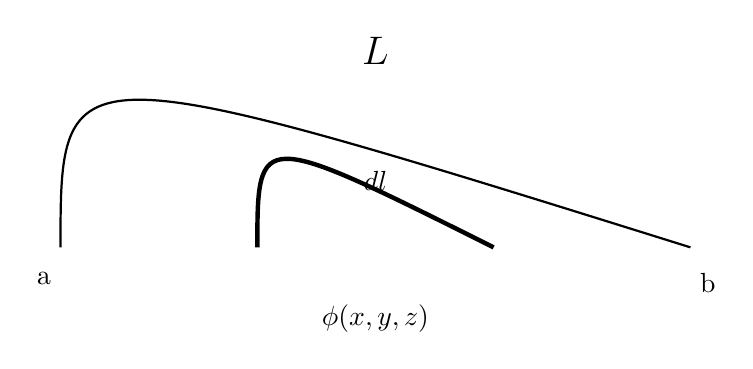
\begin{tikzpicture}[scale=1] % 整体缩放以调整整体大小

    % 1. 绘制背景:一根粗细正常的弧线 (两头有 a, b)
    % 使用贝塞尔曲线,控制点在 (0, 2.5) 处,形成自然的弧度
    \draw[thick] (-4,0) .. controls +(0, 2.5) .. (4,0);

    % 2. 在弧线中间绘制加粗的一段 (上面标注 dl)
    % 只有中间这一段使用 ultra thick
    \draw[ultra thick] (-1.5,0) .. controls +(0, 1.5) .. (1.5,0);

    % 3. 添加文字标注

    % 弧线两端的字母 a 和 b
    \node[below left] at (-4,-0.2) {a};
    \node[below right] at (4,-0.2) {b};

    % 加粗段上方的 dl
    \node[above] at (0, 0.6) {$dl$};

    % 加粗段下方的标量场符号 phi
    \node[below] at (0, -0.6) {$\phi(x,y,z)$};

    % 弧线附近的大写字母 L
    \node[align=center, font=\Large] at (0, 2.5) {$L$};

  \end{tikzpicture}
  \caption{}
  \label{fig:curve-element}
\end{figure}

将图 \ref{fig:curve-element} 中 $ a $ 到 $ b $ 的曲线段 $ L $ 上的任意一段曲线元记为 $ \d l $ ,并忽略曲线元上各点的位置变化,
则曲线元上各点的函数值可视为常数,记为 $ \phi (\bm{r}) $ 或 $ \phi (x, y, z) $。
将该位置处的函数值与曲线元长度的乘积 $ \phi (x, y, z) \d l $,从曲线段 $ L $ 的起点 $ a $ 积分到终点 $ b $,即得到沿曲线段 $ L $ 的线积分:
\begin{definition}{线积分的定义}{definition-of-line-integral}
    \begin{equation}
        \int_L \phi (x, y, z) \d l = \lim_{\max \Delta l_i \to 0} \sum_{i} \phi (\xi_i) \Delta l_i ,
    \end{equation}
    其中,曲线段 $ L $ 被划分为若干小曲线元 $ \Delta l_i $,$ \xi_i $ 为 $ \Delta l_i $ 上的某点,$ \max \Delta l_i $ 表示所有小曲线元的最大值。
\end{definition}
若取 $ \phi (x, y, z) = 1 $,则线积分即为曲线段 $ L $ 的长度。
如果 $ L $ 为闭合曲线,则称该线积分为闭合线积分,记为
\begin{equation}
    \oint_L \phi (x, y, z) \d l .
\end{equation}

\bigskip














